\documentclass[a4paper,12pt]{article}
\usepackage{setspace}
\usepackage[english]{babel}
\usepackage[utf8]{inputenc}
\usepackage{enumitem}
\usepackage{amsfonts}
\usepackage[margin=2.54cm]{geometry}
\usepackage{pdfpages}
\usepackage[utf8]{inputenc}
\usepackage[catalan]{babel}
\usepackage{graphicx,subcaption}
\usepackage{graphics}
\usepackage{lscape}
\usepackage{pdflscape}
\usepackage{float}
\usepackage{textcomp}
\usepackage{amsmath}
\usepackage{hyperref}
\usepackage{fancyvrb}
\usepackage{parskip}
\usepackage{changepage}
\usepackage{enumitem}
\usepackage{tcolorbox}
\usepackage[all]{hypcap}
\usepackage{xcolor}
\usepackage{listings}
\definecolor{green}{HTML}{228B22}
\definecolor{orange}{HTML}{FFA528}
\lstset{
    frame=tb, % draw a frame at the top and bottom of the code block
    tabsize=4, % tab space width
    showstringspaces=false, % don't mark spaces in strings
    numbers=left, % display line numbers on the left
    commentstyle=\color{green}, % comment color
    keywordstyle=\color{blue}, % keyword color
    stringstyle=\color{red}, % string color
    breaklines=true,
    numbers=left,
    xleftmargin=2em,
    framexleftmargin=1.5em,
    %postbreak=\mbox{\textcolor{red}{$\hookrightarrow$}\space},
}

\hypersetup{
    colorlinks,
    citecolor=black,
    filecolor=black,
    linkcolor=black,
    urlcolor=black
}
\title{
	\begin{center}
	\vspace{3cm}
	
\includegraphics[width=11cm, height=3cm]{images/logo_eps.png}
	\end{center}
	\begin{center}
	\line(1,0){340}
	\end{center}		
	SOFTWARE AND HARDWARE VALIDATION SYSTEMS\\
	\vspace{2mm}
	\Large Practical case 1: Verification of programs with Hoare logic and symbolic execution\\
	\line(1,0){340}
	\vspace{1.5cm}
	}

\author{Joel Aumedes Serrano - 48051307Y \\ Marc Cervera Rosell - 47980320C \vspace{1cm}}


\date{Academic course 2021 - 22\vspace{0.5cm} \\Bachelor's degree in computer engineering}
\onehalfspacing

\begin{document}
	\begin{titlepage}
		\maketitle
		\thispagestyle{empty}
	\end{titlepage}
	\cleardoublepage
	\newpage

\tableofcontents
\listoffigures
\thispagestyle{empty}

\newpage

\section{Exercise 1}
\begin{figure}[H]
    \centering
	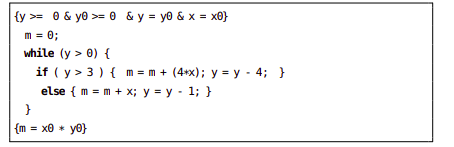
\includegraphics[scale = 0.75]{images/Screenshot from 2022-03-30 16-23-46.png}
	\caption{Exercise 1 code}
	\label{fig:code1}
\end{figure}
\justify{\textbf{\textit{Statement:}\\
Considering the algorithm (see Figure~\ref{fig:code1}) for the multiplication of two integer numbers you must:\\
1. Obtain an appropriate invariant for the loop and explain it\\
2. Perform the verification of the partial correctness of the algorithm.}} \\

\subsection{Part 1}
\begin{center}
    
    \textit{Invariant} = \{\ x = x_{0} \ \& \ y $\geq$ 0 \ \& \ m = x_{0}*(y_{0} - y) \}\ 
    
\end{center}

\begin{itemize}[label = {\clubsuit}]

    \item The value of 'x' never changes.
    \item 'y' starts $\geq$ 0, when it's '= 0', the loop ends.
    \item At each step we add "x" to "m" and we subtract 1 from "y".
    \\ When y = 0 $\rightarrow$ \mathcal{m = x_{0} * y_{0}}.
    
\end{itemize}

\pagenumbering{Arabic}
\newpage
\subsection{Part 2}
\justify{
\textit{Assignment rule:} \\
P = The same \\
$[$ m := 0 $]$ \\
while(y $>$ 0)\{ ... \} \\
Q = The same \\}

\justify{\textbf{Loop rules: \\}

\underline{Invariant initially valid (P $\rightarrow$ $\mathcal{U}$ (Inv)):} \\

\{\ y $\geq$ 0 \ \& \ y_{0} $\geq$ 0 \ \& \ y = y_{0} \ \& \ x = x_{0} \}\ \\
$\longrightarrow$ \\
\{\ x = x_{0} \ \& \ y $\geq$ 0 \ \& \ m = x_{0}*(y_{0} - y) \}\  \\ 
$[$ m := 0 $]$ \\ $\Downarrow$ \\
\{\ y $\geq$ 0 \ \& \ y_{0} $\geq$ 0 \ \& \ y = y_{0} \ \& \ x = x_{0} \}\ \\
$\longrightarrow$ \\
\{\ x = x_{0} \ \& \ y $\geq$ 0 \ \& \ 0 = x_{0}*(y_{0} - y) \}\ }
\newline

\begin{itemize}[label = {\checkmark}]
    \item x = $x_{0}$ is in P.
    \item y = $y_{0}$ is in P.
    \item ($y_{0}$ - y) = 0 because y = $y_{0}$ in P $\Rightarrow$ m = 0 = 0 * 0.
\end{itemize} \\

\newpage

\underline{Invariant preserved (\{ Inv \ \& \ b \} \[ \] $\rightarrow$ \{ Inv \}):} \\

$[$ m := 0 $]$ \\
\{\ $x = x_{0}$ \ \& \ y $\geq$ 0 \ \& \ m = $x_{0}$*$(y_{0}$ - y) \ y $>$ 0 \}\ \\

\begin{figure}[H]
    \centering
	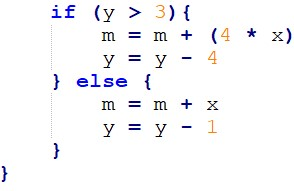
\includegraphics[scale = 1.0]{images/loop code.jpg}
	\caption{Loop code}
	\label{fig:loopCode}
\end{figure}

\textit{Quick remember:} \\
Inv = \{\ $x = x_{0}$ \ \& \ y $\geq$ 0 \ \& \ $m = x_{0}*(y_{0} - y)$ \}\

\subsubsection{Conditional rule $\rightarrow$ True side}
\{\ $x = x_{0}$ \ \& \ y $\geq$ 0 \ \& \ m = $x_{0}$*$(y_{0}$ - y) \ y $>$ 0 \ \& \ y $>$ 3 \}\ \\
$[$ m := 0 $||$ m := m + (4 * x) $||$ y := y - 4 $]$ (More than one assignment rule) \\
\{\ $x = x_{0}$ \ \& \ y $\geq$ 0 \ \& \ $m = x_{0}*(y_{0} - y)$ \}\ \\

\textit{Exit rule (P $\rightarrow$ $\mathcal{U}$ (Q)):} \\
\{\ $x = x_{0}$ \ \& \ y $\geq$ 0 \ \& \ m = $x_{0}$*$(y_{0}$ - y) \ y $>$ 0 \ \& \ y $>$ 3 \}\ \\
$\longrightarrow$ \\
\{ $x = x_{0}$ \ \& \ y - 4 $\geq$ 0 \ \& \ 0 + 4 * x = $x_{0} * (y_{0} - (y - 4))$ \}

\begin{itemize}[label = {\checkmark}]
    \item x = $x_{0}$ is in P.
    \item y = y $>$ 3 + y $\geq$ 4 $\rightarrow$ y- 4 $\geq$ 0.
    \item 4 * x = $x_{0}$ * $y_{0}$ - $x_{0}$ * y + 4 * x $\rightarrow$ 4 * x = $x_{0}$ * ($y_{0}$ - y) + 4 * x $\Rightarrow$ m = 0.
\end{itemize} \\
\newpage
\subsubsection{Conditional rule $\rightarrow$ False side}
\{\ $x = x_{0}$ \ \& \ y $\geq$ 0 \ \& \ m = $x_{0}$*$(y_{0}$ - y) \ y $>$ 0 \ \& \ !(y $>$ 3) \}\ \\
$[$ m := 0 $||$ m := m + x $||$ y := y - 1 $]$ (More than one assignment rule) \\

\textit{Exit rule (P $\rightarrow$ $\mathcal{U}$ (Q)):} \\
\{\ $x = x_{0}$ \ \& \ y $\geq$ 0 \ \& \ m = $x_{0}$*$(y_{0}$ - y) \ y $>$ 0 \ \& \ !(y $>$ 3) \}\ \\
$\longrightarrow$ \\
\{ $x = x_{0}$ \ \& $y - 1$ $\geq$ 0 \ \& \ 0 + x = $x = x_{0}$ * ($y_{0}$ - y + 1) \} \\
\begin{itemize}[label = {\checkmark}]
    \item x = $x_{0}$ is in P.
    \item y $\geq$ 0 is in P and y $\geq$ 1.
    \item 0 + x = $x = x_{0}$ * ($y_{0}$ - y + 1) $\rightarrow$ 0 + $x_{0}$ = $x_{0}$ * ($y_{0}$ - y) + $x_{0}$ $\Rightarrow$ m = 0.
\end{itemize} \\

\underline{Use case (\{ Inv \ \& \ !b \} \[ \] $\rightarrow$ \{ Q \}):} \\

\{\ $x = x_{0}$ \ \& \ y $\geq$ 0 \ \& \ m = $x_{0}$*$(y_{0}$ - y) \ !(y $>$ 0) \}\ \\
$[$ m := 0 $]$  (Assignment rule)\\
\{ m = $x_{0}$ * $y_{0}$ \} \\

\textit{Exit rule:}\\
\{\ $x = x_{0}$ \ \& \ y $\geq$ 0 \ \& \ m = $x_{0}$*$(y_{0}$ - y) \ !(y $>$ 0) \}\ \\
$\longrightarrow$ \\
$[$ m := 0 $]$ \\
\{ m = $x_{0}$ * $y_{0}$ \} \\
$\Downarrow$ \\
\{\ $x = x_{0}$ \ \& \ y $\geq$ 0 \ \& \ m = $x_{0}$*$(y_{0}$ - y) \ !(y $>$ 0) \}\ \\
$\longrightarrow$ \\
\{ m = $x_{0}$ * $y_{0}$ \} \\
\begin{itemize}[label = {\checkmark}]
    \item (!(y $>$ 0) \ \& \ y $\geq$ 0) $\rightarrow$ y = 0 $\Rightarrow$ m = $x_{0}$ * ($y_{0}$ - 0) = $x_{0}$ * $y_{0}$
\end{itemize} \\
\newpage

\section{Exercise 2}
\begin{figure}[H]
    \centering
	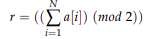
\includegraphics[scale = 1.0]{images/formula.png}
	\caption{Exercise 2 formula}
	\label{fig:formula1}
\end{figure}
\begin{figure}[H]
    \centering
	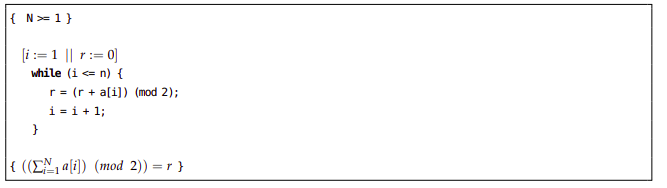
\includegraphics[scale = 0.70]{images/codi.png}
	\caption{Exercise 2 code}
	\label{fig:code2}
\end{figure}
\justify{\textbf{\textit{Statement:\\}
Verify the algorithm of the Figure~\ref{fig:code2} for computing the parity of the sum of the elements of an array a[N] with N \textbf{$\geq 0$} and storing it in the result variable r. You must:\\
1. Obtain an appropriate invariant for the loop and explain it.\\
2. Perform the verification of the partial correctness of the algorithm.}}
\subsection{Part 1}
\justify{To perform the validation, we're going to use the following invariant formula: \\}
\begin{center}
    
    \textit{Invariant} =  \{\ [(((a[i] + a[i + 1]) \% 2 = 0) \longrightarrow (r = 0 \wedge (a[i] + a[i + 1] = 2n))) \vee (((a[i] + a[i + 1]) \% 2 > 0) \longrightarrow (r > 0 \vee  (a[i] + a[i + 1]) = (2n + 1)))] \wedge ((summation(i, n, a)) \% 2 = r) \}\
    
\end{center}

\begin{itemize}[label = {\clubsuit}]

    \item The first logical disjunction, is a tautology, therefore, it always will be true. It's a tautology , because a number, always, is odd or even. That is, the parity of a number is a binary question. Either it's odd or it's even.
    \item If we go one step further into the tautology, we will see that the first part (left part of the disjunction), represents the even numbers because, we can see that when we apply the $\%2$, the result is 0 and r i 0 too.
    \item The right part of the disjunction represents the odd numbers.
    \item The predicate \textit{summation(i, n, a)}, represents the summation of the array elements. Finally, once the summation is done, we apply the modulus and we match this with r.
    
    \begin{itemize}
    
        \item The parameter i of the predicate, is the lower limit.
        \item The parameter n of the predicate is the higher limit.
        \item The parameter a of the predicate, is the array.
        
    \end{itemize}
    
\end{itemize}

\subsection{Part 2}
\justify{To simplify the document writing, we're going to apply directly the multiple assignment and exit rules. Anyway we will specify where are applied.}

\justify{As we can see in Figure~\ref{fig:code2} the assignment rule is already applied at the beginning (before the loop), hence we are able to start with the loop rules and the partial verification. \\}

\textbf{Loop rules:\\}

\underline{Invariant initially valid (P $\rightarrow$ $\mathcal{U}$ (Inv)):}
\\

\justify{ \{\ n \geq 1 \}\ \\
\longrightarrow \\
 \{\ [(((a[1] + a[2]) \% 2 = 0) \longrightarrow (0 = 0 \wedge (a[1] + a[2] = 2n))) \vee (((a[1] + a[2]) \% 2 > 0) \longrightarrow (0 > 0 \wedge  (a[1] + a[2]) = (2n + 1)))] \wedge ((summation(1, n, a)) \% 2 = 0) \}\ \\}
 
\justify{Initially, \textit{r = 0}, so that means that we're talking about an even number. Hence, "(a[1] + a[2] = 2n" is true. Beside, if we take a look after applying the exit rule to the invariant, it's the only logical thing since in the disjunction we can observe "0 $>$ 0", and that's completely false. Therefore as 0 is not greater than 0, the conjunction is false. So that something implies something false $(X \rightarrow F)$ becomes true, the only way is to evaluate to false the left side. Thus confirming that we've said at the beginning (we're talking about an even number). At this point we've evaluated to true the disjunction with a logical reasoning. now we've to make true the global conjunction. As we've said previously, we're talking about an even number, so the summation of the array elements among two limits module 2 has to be 0, and taking a look at the predicate clause we can confirm that. Finally if we want to express what we've in logical variables: $(True \vee False) \wedge True$.}
\newpage
\underline{Invariant preserved (\{ Inv \ \& \ b \} \[ \] $\rightarrow$ \{ Inv \}):} \\

\{\ [(((a[i] + a[i + 1]) \% 2 = 0) \longrightarrow (r = 0 \wedge (a[i] + a[i + 1] = 2n))) \vee (((a[i] + a[i + 1]) \% 2 > 0) \longrightarrow (r > 0 \vee  (a[i] + a[i + 1]) = (2n + 1)))] \wedge ((summation(i, n, a)) \% 2 = r) \wedge ($i \leq n$) \}\
\longrightarrow \\
\{\ [(((a[i + 1] + a[i + 2]) \% 2 = 0) \longrightarrow (((r + a[i + 1])\% 2) = 0 \wedge (a[i + 1] + a[i + 2] = 2n))) \vee (((a[i + 1] + a[i + 2]) \% 2 > 0) \longrightarrow (((r + a[i + 1])\% 2) > 0 \vee  (a[i + 1] + a[i + 2]) = (2n + 1)))] \wedge ((summation(i + 1, n, a)) \% 2 = (r + a[i + 1]) \% 2) \}\
\\

\justify{We've applied the assignment rule and the exit rule at the right part of the implication. The update is the code of the inside of the loop. The update is:}
\begin{center}
    
     $[$ r = (r + a[i] \% 2 ) \ $||$ \  i = i + 1 $]$
    
\end{center}
\justify{As we've said at first part of the exercise, the disjunction is a tautology, then it always be true. The predicate part is true too because to know the parity of a sum, we need the \textit{r} of the previous sum. In other words, to know the parity of a sum "p", where "p" > 1 we need the sum parity of the previous elements of the array. To watch it more graphically, see Figure~\ref{fig:Graphic} }

\begin{figure}[H]
    \centering
    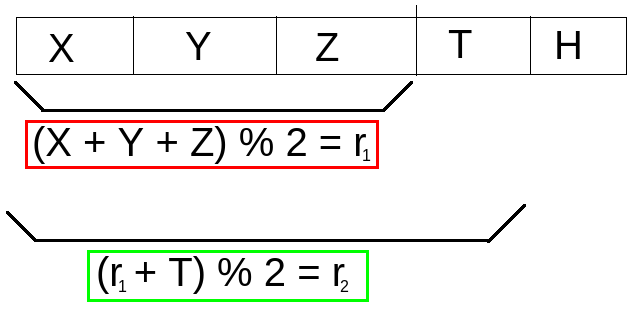
\includegraphics[scale = 0.75]{images/graphic.png}
    \caption{Graphical representation of the correctness of the predicate after a random iteration.}
    \label{fig:Graphic}
\end{figure}

\newpage

\underline{Use case (\{ Inv \ \& \ !b \} \[ \] $\rightarrow$ \{ Q \}):} \\

\{\ [(((a[i] + a[i + 1]) \% 2 = 0) \longrightarrow (r = 0 \wedge (a[i] + a[i + 1] = 2n))) \vee (((a[i] + a[i + 1]) \% 2 > 0) \longrightarrow (r > 0 \vee  (a[i] + a[i + 1]) = (2n + 1)))] \wedge ((summation(i, n, a)) \% 2 = r) \wedge (i > n) \}\ \\
\longrightarrow \\
\{ ((summation(i, n, a)) \% 2 = r) \}
\\

\justify{As there's no more code to execute, the invariant formula with the negated iteration condition implies the post-condition (without applying any more rule) and as we can find the post-condition above, the implication is true.}
\end{document}
